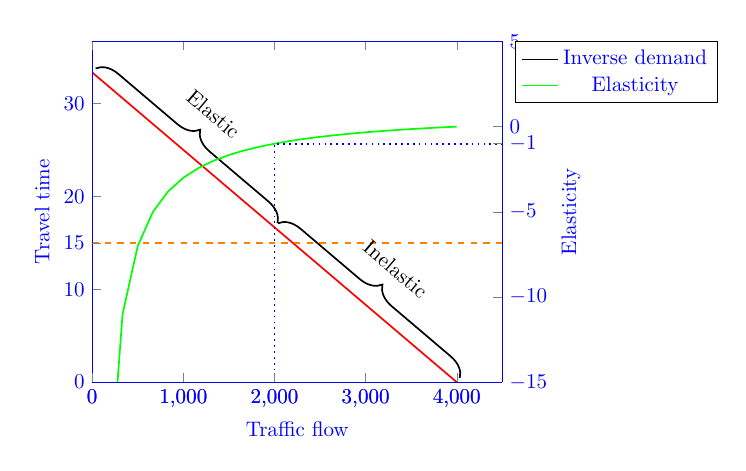
\begin{tikzpicture}[
  blue,
  scale=0.76,
  declare function = {
    demand(\v) = 100/3 - \v / 120 ;
    elasv(\v) = 1 - 4000 / \v ;
  }
]
  \begin{axis}[
      xlabel={Traffic flow},
      ylabel={Travel time},
      axis y line* = left, % the '*' avoids arrow heads
      domain=0:4000,
      xmin=0,
      xmax=4500,
      extra y ticks={15},
      ymin=0,
      axis on top,
    ]
    \addplot[red, thick, no marks] {demand(x)}; \label{plot_demand}
    \addplot[dashed, thick, orange, domain=0:4500] {15} ;
    \draw [
      thick,
      decorate, 
      decoration={brace, amplitude=10pt, raise=2.5pt}, 
      black,
    ] (0, {demand(0)}) --  (2000, {demand(2000)}) node [above, midway, sloped, yshift=15] {Elastic};
    \draw [
      thick,
      decorate, 
      decoration={brace, amplitude=10pt, raise=2.5pt}, 
      black,
    ] (2000, {demand(2000)}) -- (4000, {demand(4000)}) node [above, midway, sloped, yshift=15] {Inelastic};
  \end{axis}
  
  \begin{axis}[
      ylabel={Elasticity},
      axis y line* = right, % the '*' avoids arrow heads
      domain=0:4000,
      xmin=0,
      xmax=4500,
      ymin=-15,
      ymax=5,
      extra y ticks = {-1},
      axis on top,
      legend pos=outer north east,
    ]
    \addlegendimage{/pgfplots/refstyle=plot_demand}\addlegendentry{Inverse demand} ;
    \addplot+[green, thick, no marks] {elasv(x)};
    \addlegendentry{Elasticity}
    \draw[thick, dotted] {
      (2000, \pgfkeysvalueof{/pgfplots/ymin}) --
      (2000, {elasv(2000)}) -- (\pgfkeysvalueof{/pgfplots/xmax}, {elasv(2000)})
    };
  \end{axis}
\end{tikzpicture}
